%LTeX: language=it

\begin{figure}[H]
    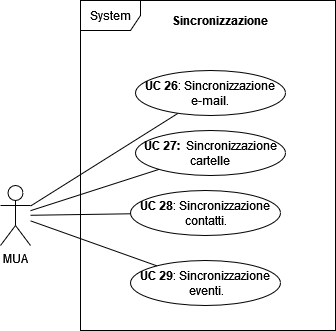
\includegraphics[width=0.55\textwidth]{sections/uc_imgs/UC-sincronizzazione.png}
    \centering
    \caption{Casi d'uso relativi alla sincronizzazione.}
\end{figure}

\subsection{UC 26 - Sincronizzazione e-mail} \label{sec:UC26}
    
    \begin{itemize}
        \item \textbf{Attore principale}: MUA;
        \item \textbf{Descrizione}: il MUA richiede la sincronizzazione con le e-mail del sistema;
        \item \textbf{Precondizioni}: l’account che il MUA gestisce è registrato nel sistema, ha una connessione aperta con il sistema ed è autenticato;
        \item \textbf{Postcondizioni}: le e-mail sono state sincronizzate;
        \item \textbf{Scenario principale}:
            \begin{enumerate}
                \item il MUA trasmette l'id dell'account (\hyperref[sec:UC26.1]{UC26.1});
                \item il MUA trasmette gli id delle e-mail da aggiornare (\hyperref[sec:UC26.2]{UC 26.2});
                \item il MUA trasmette le proprietà delle e-mail da aggiornare (\hyperref[sec:UC26.3]{UC 26.3});
                \item il sistema invia al MUA gli aggiornamenti;
            \end{enumerate}
        \item \textbf{Inclusioni}: nessuna;
        \item \textbf{Generalizzazioni}: nessuna;
        \item \textbf{Estensioni}: nessuna;
    \end{itemize}

    \begin{figure}[H]
        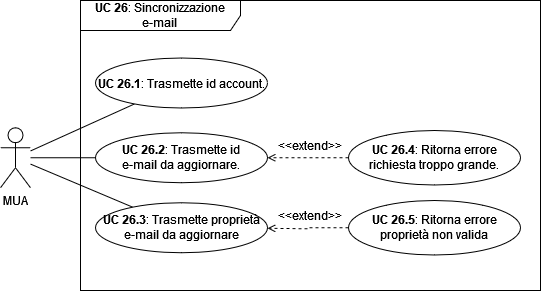
\includegraphics[width=0.85\textwidth]{sections/uc_imgs/UC26.png}
        \centering
        \caption{Sottocasi d'Uso di UC 26}
    \end{figure}

    \subsubsection{UC 26.1 - Trasmette id account} \label{sec:UC26.1}
    \begin{itemize}
        \item \textbf{Attore principale}: MUA;
        \item \textbf{Descrizione}: il MUA invia al sistema l'id dell'account associato all'utente;
        \item \textbf{Precondizioni}: il MUA sta usando la funzionalità di sincronizzazione e-mail;
        \item \textbf{Postcondizioni}: il sistema conosce l'id dell'account;
        \item \textbf{Scenario principale}:
            \begin{enumerate}
                \item il MUA trasmette l'id dell'account associato all'utente al sistema;
            \end{enumerate}
        \item \textbf{Inclusioni}: nessuna;
        \item \textbf{Generalizzazioni}: nessuna;
        \item \textbf{Estensioni}: nessuna;
    \end{itemize}

    \subsubsection{UC 26.2 - Trasmette id e-mail da aggiornare} \label{sec:UC26.2}
    \begin{itemize}
        \item \textbf{Attore principale}: MUA;
        \item \textbf{Descrizione}: il MUA invia al sistema gli id delle e-mail da aggiornare;
        \item \textbf{Precondizioni}: il MUA sta usando la funzionalità di sincronizzazione delle e-mail;
        \item \textbf{Postcondizioni}: il sistema conosce gli id delle e-mail da aggiornare;
        \item \textbf{Scenario principale}:
            \begin{enumerate}
                \item il MUA trasmette gli id delle e-mail da aggiornare;
            \end{enumerate}
        \item \textbf{Inclusioni}: nessuna;
        \item \textbf{Generalizzazioni}: nessuna;
        \item \textbf{Estensioni}:
            \begin{enumerate}[label=\alph*.]
                \item la quantità di e-mail da aggiornare supera la quantità massima di richieste al server:
                \begin{enumerate}[label=\arabic*.]
                    \item il sistema ritorna un errore al MUA di richiesta troppo grande (\hyperref[sec:UC26.4]{UC 26.4}).
                \end{enumerate}
            \end{enumerate}
    \end{itemize}


    \subsubsection{UC 26.3 - Trasmette proprietà e-mail da aggiornare} \label{sec:UC26.3}
    \begin{itemize}
        \item \textbf{Attore principale}: MUA;
        \item \textbf{Descrizione}: il MUA invia al sistema le proprietà delle e-mail da aggiornare;
        \item \textbf{Precondizioni}: il MUA sta usando la funzionalità di sincronizzazione delle e-mail;
        \item \textbf{Postcondizioni}: il sistema conosce quali sono le proprietà delle e-mail da aggiornare;
        \item \textbf{Scenario principale}:
            \begin{enumerate}
                \item il MUA trasmette le proprietà delle e-mail da aggiornare;
            \end{enumerate}
        \item \textbf{Inclusioni}: nessuna;
        \item \textbf{Generalizzazioni}: nessuna;
        \item \textbf{Estensioni}:
            \begin{enumerate}[label=\alph*.]
                \item le proprietà delle e-mail da aggiornare non sono valide:
                \begin{enumerate}[label=\arabic*.]
                    \item il sistema ritorna un errore al MUA di proprietà non valida (\hyperref[sec:UC26.5]{UC 26.5}).
                \end{enumerate}
            \end{enumerate}
    \end{itemize}


    \subsubsection{UC 26.4 - Ritorna errore richiesta troppo grande} \label{sec:UC26.4}
    \begin{itemize}
        \item \textbf{Attore principale}: MUA;
        \item \textbf{Descrizione}: il MUA riceve l'errore che la quantità delle e-mail da aggiornare supera la quantità massima di richieste al server;
        \item \textbf{Precondizioni}: il MUA ha inviato gli id delle e-mail da aggiornare;
        \item \textbf{Postcondizioni}: il sistema non invia gli aggiornamenti e il MUA viene notificato che il numero delle e-mail da aggiornare è eccessivo;
        \item \textbf{Scenario principale}:
            \begin{enumerate}
                \item il sistema verifica la quantità di richieste;
                \item il sistema rileva che il numero di richieste supera la soglia massima consentita;
                \item il sistema non invia gli aggiornamenti e notifica il MUA dell'eccesso di richieste;
            \end{enumerate}
        \item \textbf{Inclusioni}: nessuna;
        \item \textbf{Generalizzazioni}: nessuna;
        \item \textbf{Estensioni}: nessuna.
    \end{itemize}

    \subsubsection{UC 26.5 - Ritorna errore proprietà non valida} \label{sec:UC26.5}
    \begin{itemize}
        \item \textbf{Attore principale}: MUA;
        \item \textbf{Descrizione}: il MUA riceve l'errore che la proprietà dell'e-mail da aggiornare non è valida;
        \item \textbf{Precondizioni}: il MUA ha inviato la proprietà dell'e-mail da aggiornare;
        \item \textbf{Postcondizioni}: il sistema non invia gli aggiornamenti e il MUA viene notificato che la proprietà dell'e-mail da aggiornare non è valida;
        \item \textbf{Scenario principale}:
            \begin{enumerate}
                \item il sistema verifica la validità della proprietà trasmessa e trova un errore;
                \item il sistema non invia gli aggiornamenti e notifica il MUA dell'errore;
            \end{enumerate}
        \item \textbf{Inclusioni}: nessuna;
        \item \textbf{Generalizzazioni}: nessuna;
        \item \textbf{Estensioni}: nessuna.
    \end{itemize}